\documentclass[crop,tikz]{standalone}
\usepackage{amsmath}
\usetikzlibrary{positioning}
\usetikzlibrary{shapes}


\begin{document}
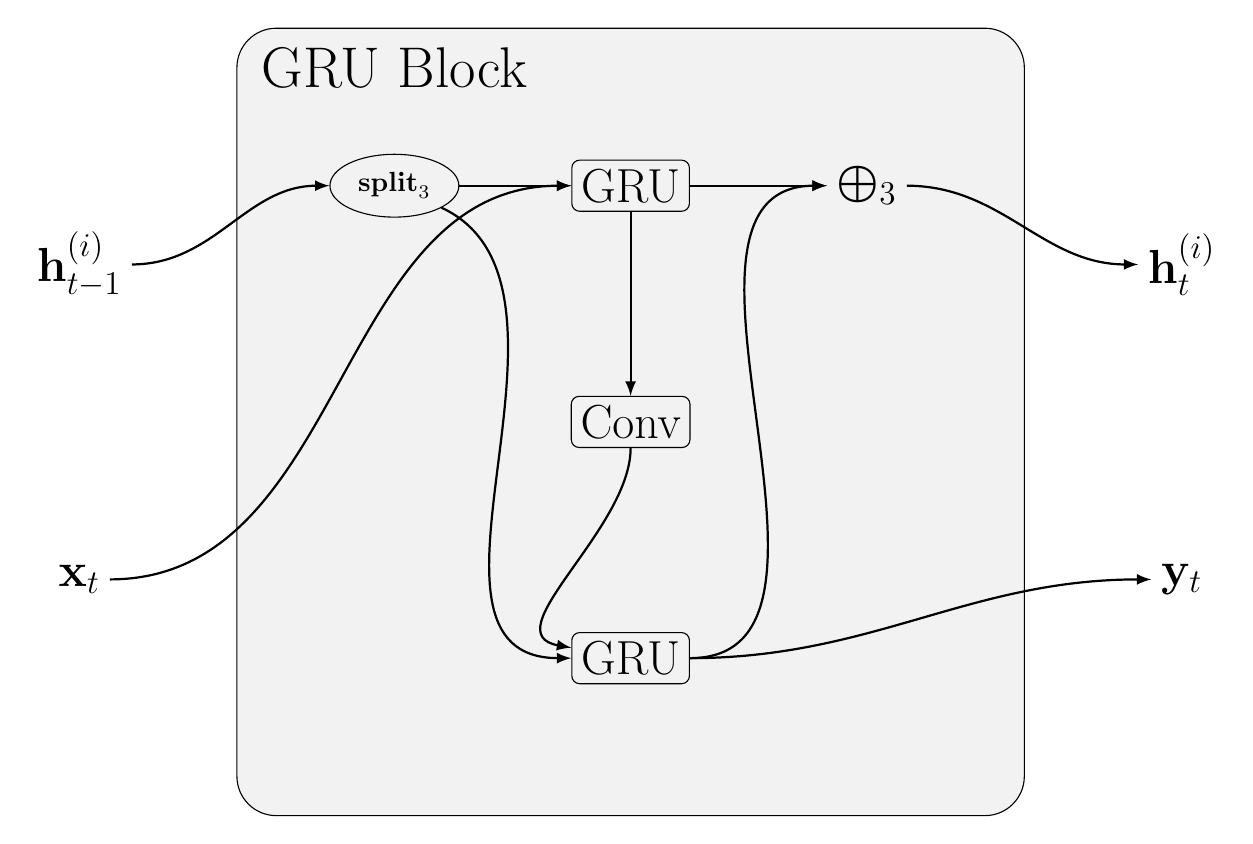
\begin{tikzpicture}[
    node distance=3cm
]
    \draw[rounded corners=0.5cm, fill=black!5, draw=black] (-5, -5) rectangle (5, 5);
    \node (title) at (-3, 4.5) {\huge GRU Block};
    \node (states) at (-7, 2) {\LARGE$\mathbf{h}^{(i)}_{t-1}$};
    \node (x) at (-7, -2) {\LARGE$\mathbf{x}_t$};
    
    \node[ellipse, draw=black] (split) at (-3, 3) {$\text{\textbf{split}}_{3}$};
    \draw[in=180, out=0, -latex, thick] (states) to (split);
    % \node (concat) [right of=split] {\LARGE$\boldsymbol{\oplus}_3$};
    % \draw[in=180, out=0, -latex, thick] (split) to (concat);
    % \draw[in=180, out=0, -latex, thick] (x) to (concat);
    
    \node[rectangle, draw=black, rounded corners=0.1cm] (gru1) [right of=split] {\LARGE GRU};
    \draw[-latex, thick] (split) to (gru1);
    \draw[in=180, out=0, -latex, thick] (x) to (gru1);

    
    \node[rectangle, draw=black, rounded corners=0.1cm] (conv) [below of=gru1] {\LARGE Conv};
    \draw[-latex, thick] (gru1) to (conv);
    
    \node[rectangle, draw=black, rounded corners=0.1cm] (gru2) [below of=conv] {\LARGE GRU};
    % \node (concat2) [left of=gru2] {\LARGE$\boldsymbol{\oplus}_3$};
    \draw[-latex, thick, out=-25, in=180] (split) to (gru2);
    \draw[-latex, thick, out=270, in=170] (conv) to (gru2);
    % \draw[-latex, thick] (concat2) to (gru2);
    
    \node (concat states) [right of=gru1] {\LARGE$\boldsymbol{\oplus}_3$};
    \node (output states)  at (7, 2) {\LARGE $\mathbf{h}^{(i)}_{t}$};
    \node (output)  at (7, -2) {\LARGE $\mathbf{y}_{t}$};
    
    \draw[-latex, thick] (gru1) to (concat states);
    \draw[-latex, thick, in=180, out=0] (gru2) to (concat states);
    \draw[-latex, thick, out=0, in=180] (concat states) to (output states);
    \draw[-latex, thick, out=0, in=180] (gru2) to (output);
    
\end{tikzpicture}
\end{document}